\subsection{Fake Source Injection for DIA}
\subsubsection{Selection of a data subset}

In this subsection we select a portion of the observations processed by the DRP pipelines that include DIA, and run some simple analysis checks on the data contents. There are many fields being observed with LSSTComCam that span a large portion of the southern hemisphere accessible sky at this time of year (fall 2024).

From these, we make a selection, choosing a very well covered field in all bandpasses. In Fig.\ref{ref:deep_df} we show the full coverage of LSSTComCam up to current date.

\begin{figure}
    \centering
    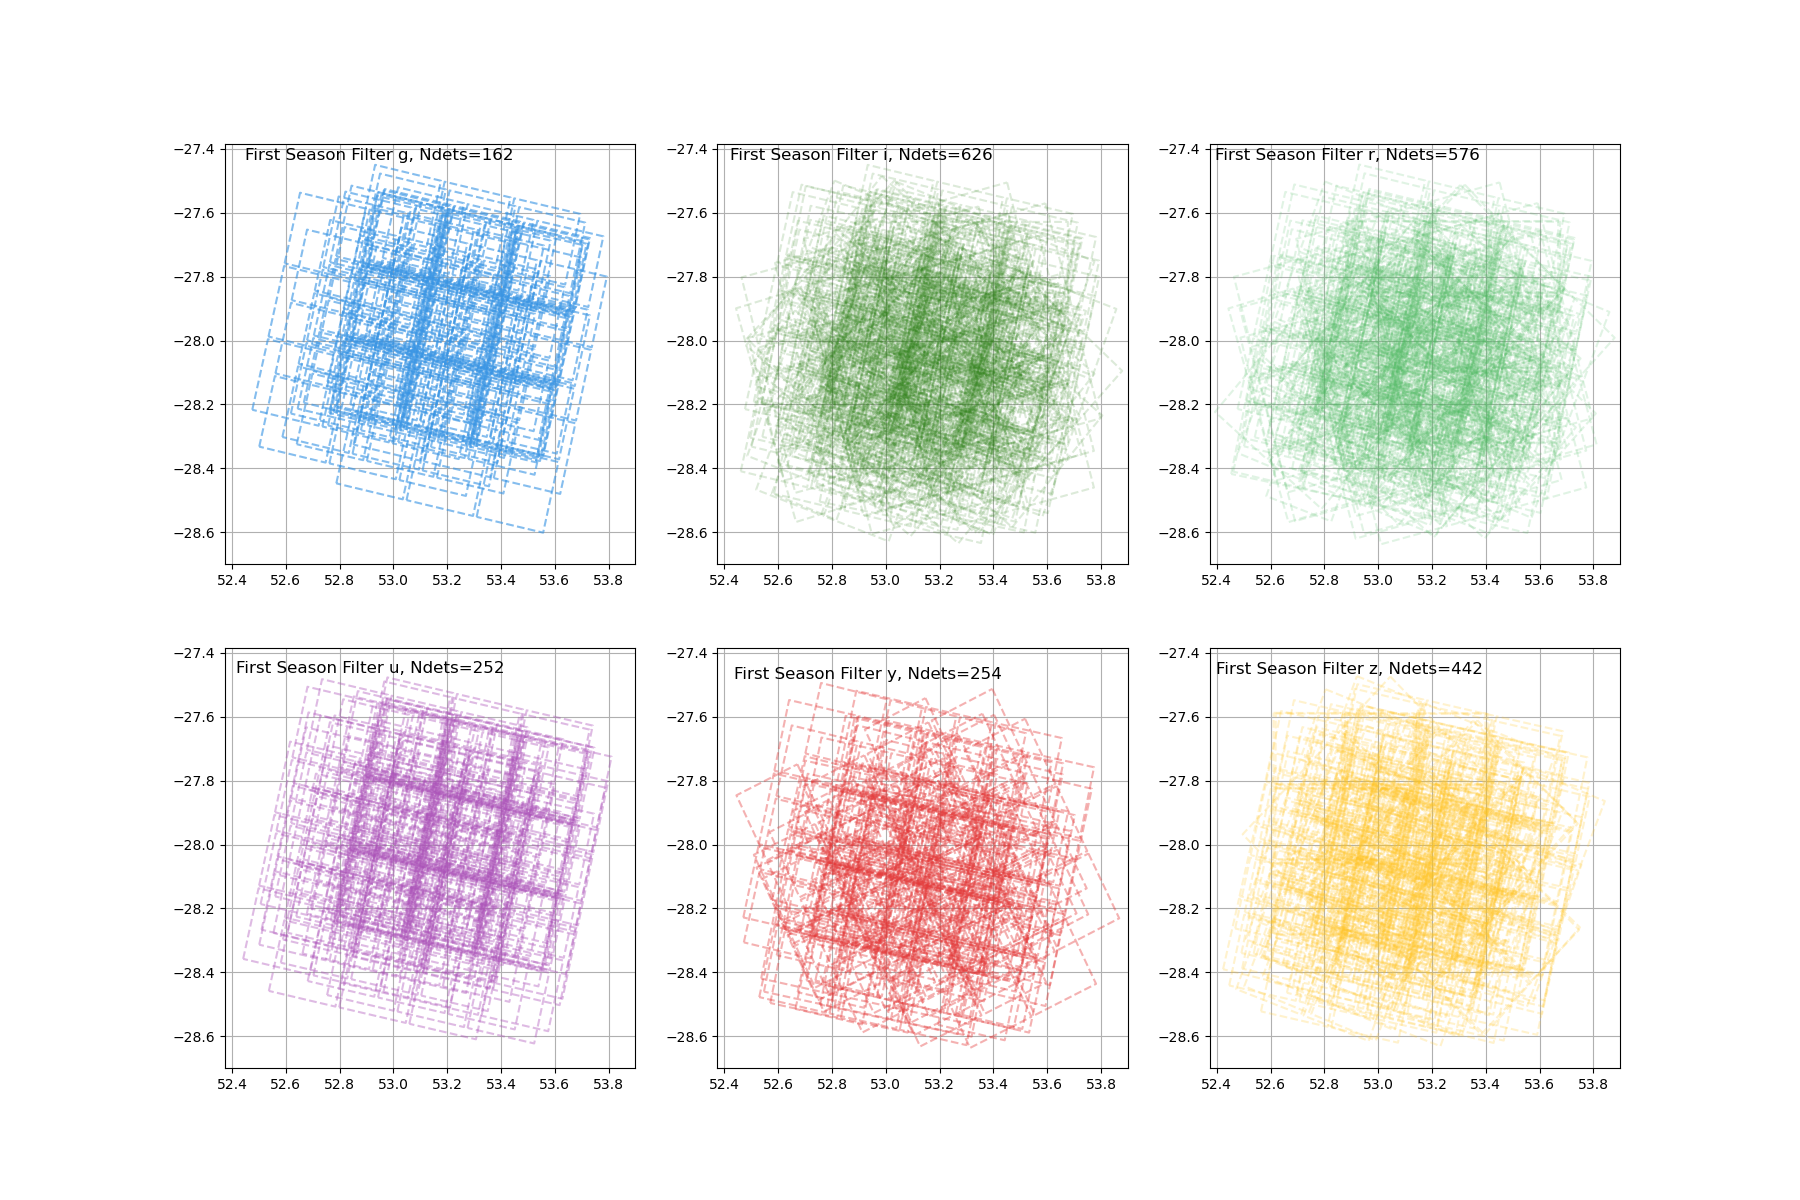
\includegraphics[width=0.95\linewidth]{dia/figures/deep_df_chip_observations.png}
    \caption{The full LSSTComCam set of observations overlapping the chosen field and with elevation > 45 above the horizon.}
    \label{fig:deep_df}
    
\end{figure}

In Fig~\ref{fig:sampled_df_chip_observations} we apply a first cut on the observations, to narrow our visit list to a total of 24 visits. This cut involves a zenith distance of less than 45 degrees, as well as some technical parameters, derived from the nominal DRP DIA performance (ratio of PSF between template and science, as well as Kernel basis condition number). 

\begin{figure}
    \centering
    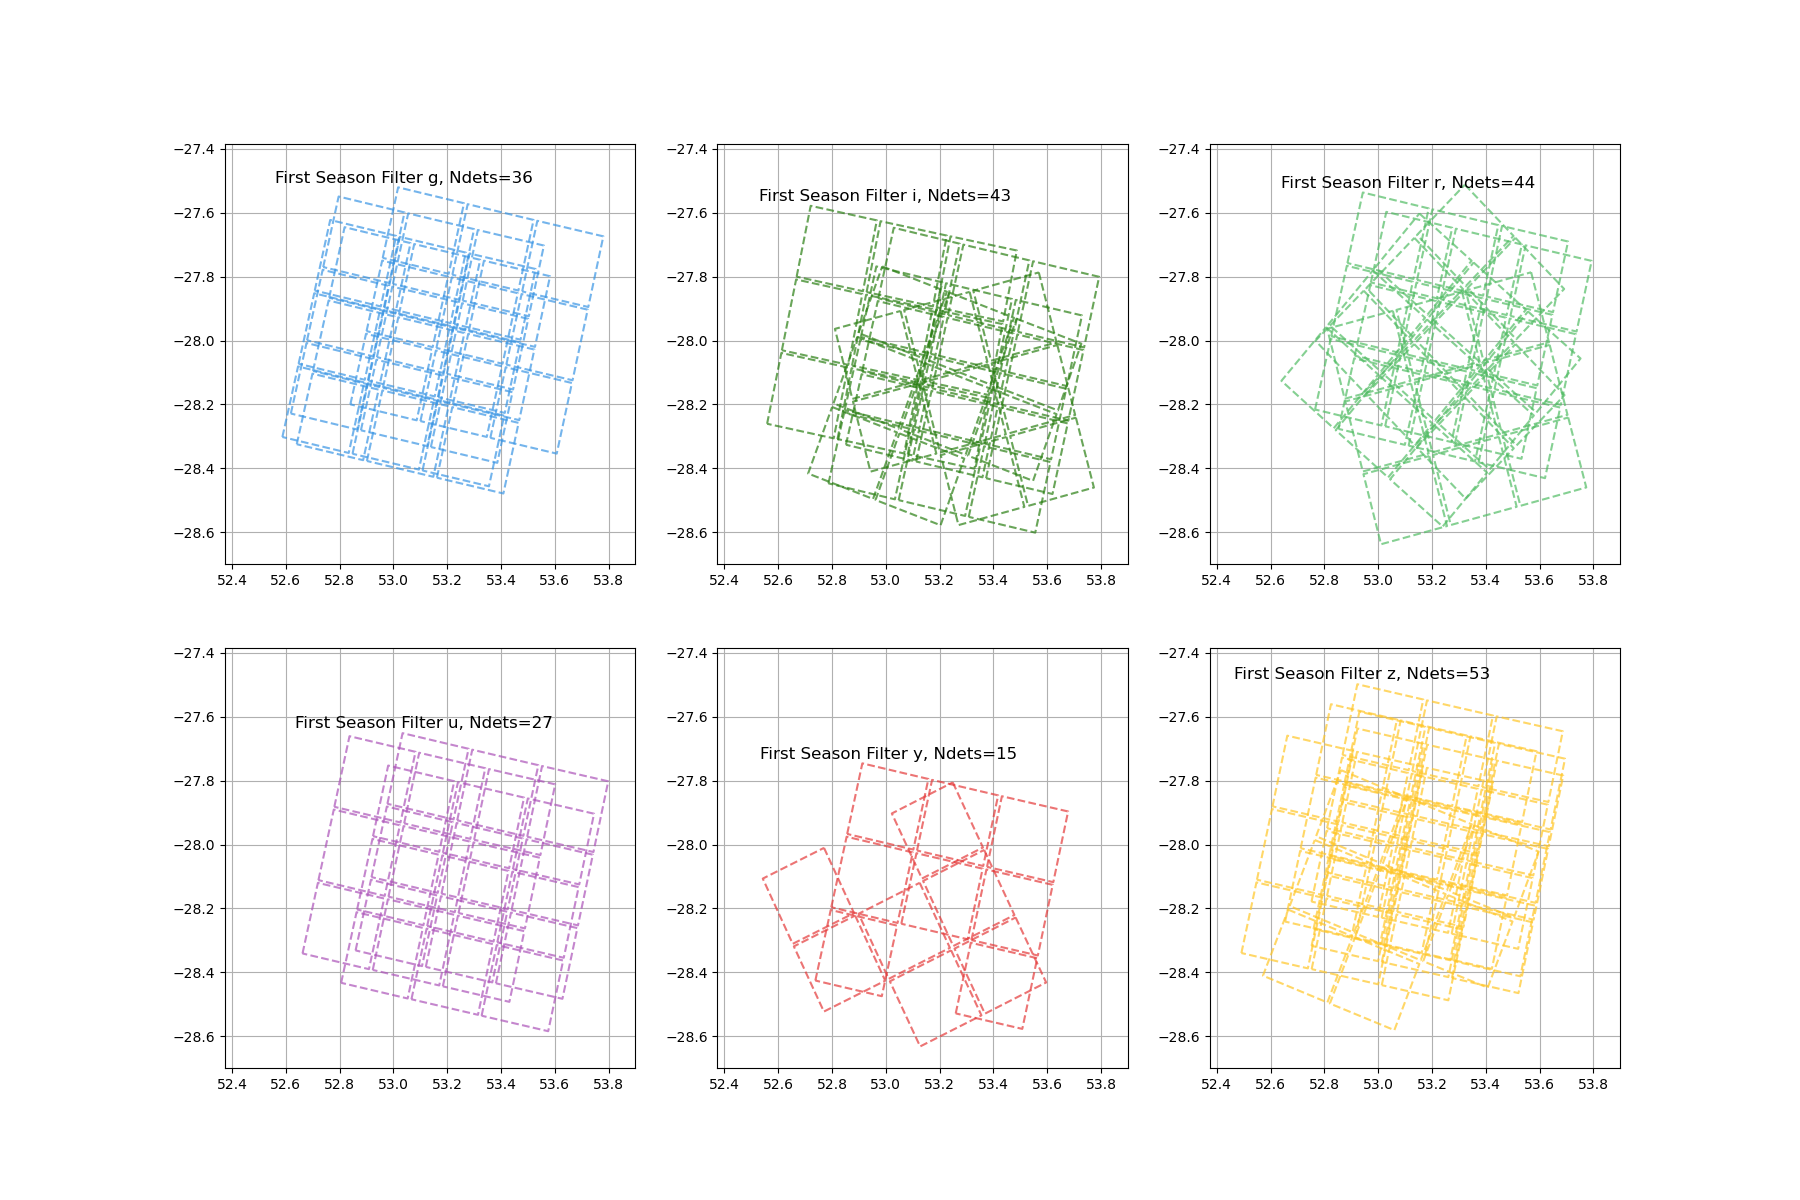
\includegraphics[width=0.95\linewidth]{dia/figures/sampled_df_chip_observations.png}
    \caption{The selection of CCDs for fake injection processing.}
    \label{fig:sampled_df_chip_observations}
\end{figure}


We create a catalog of fakes for this sample of visits, by creating position and magnitudes of the synthetic sources to be injected. In Fig~\ref{fig:sampled_df_chip_observations_plusfakes} we show the fake distribution per chip in our selection. We use sources that are possibly extended, and choose the fake location in its sourroundings. The magnitudes are chosen so they are within 1.5 magnitudes of the selected source host.

\begin{figure}
    \centering
    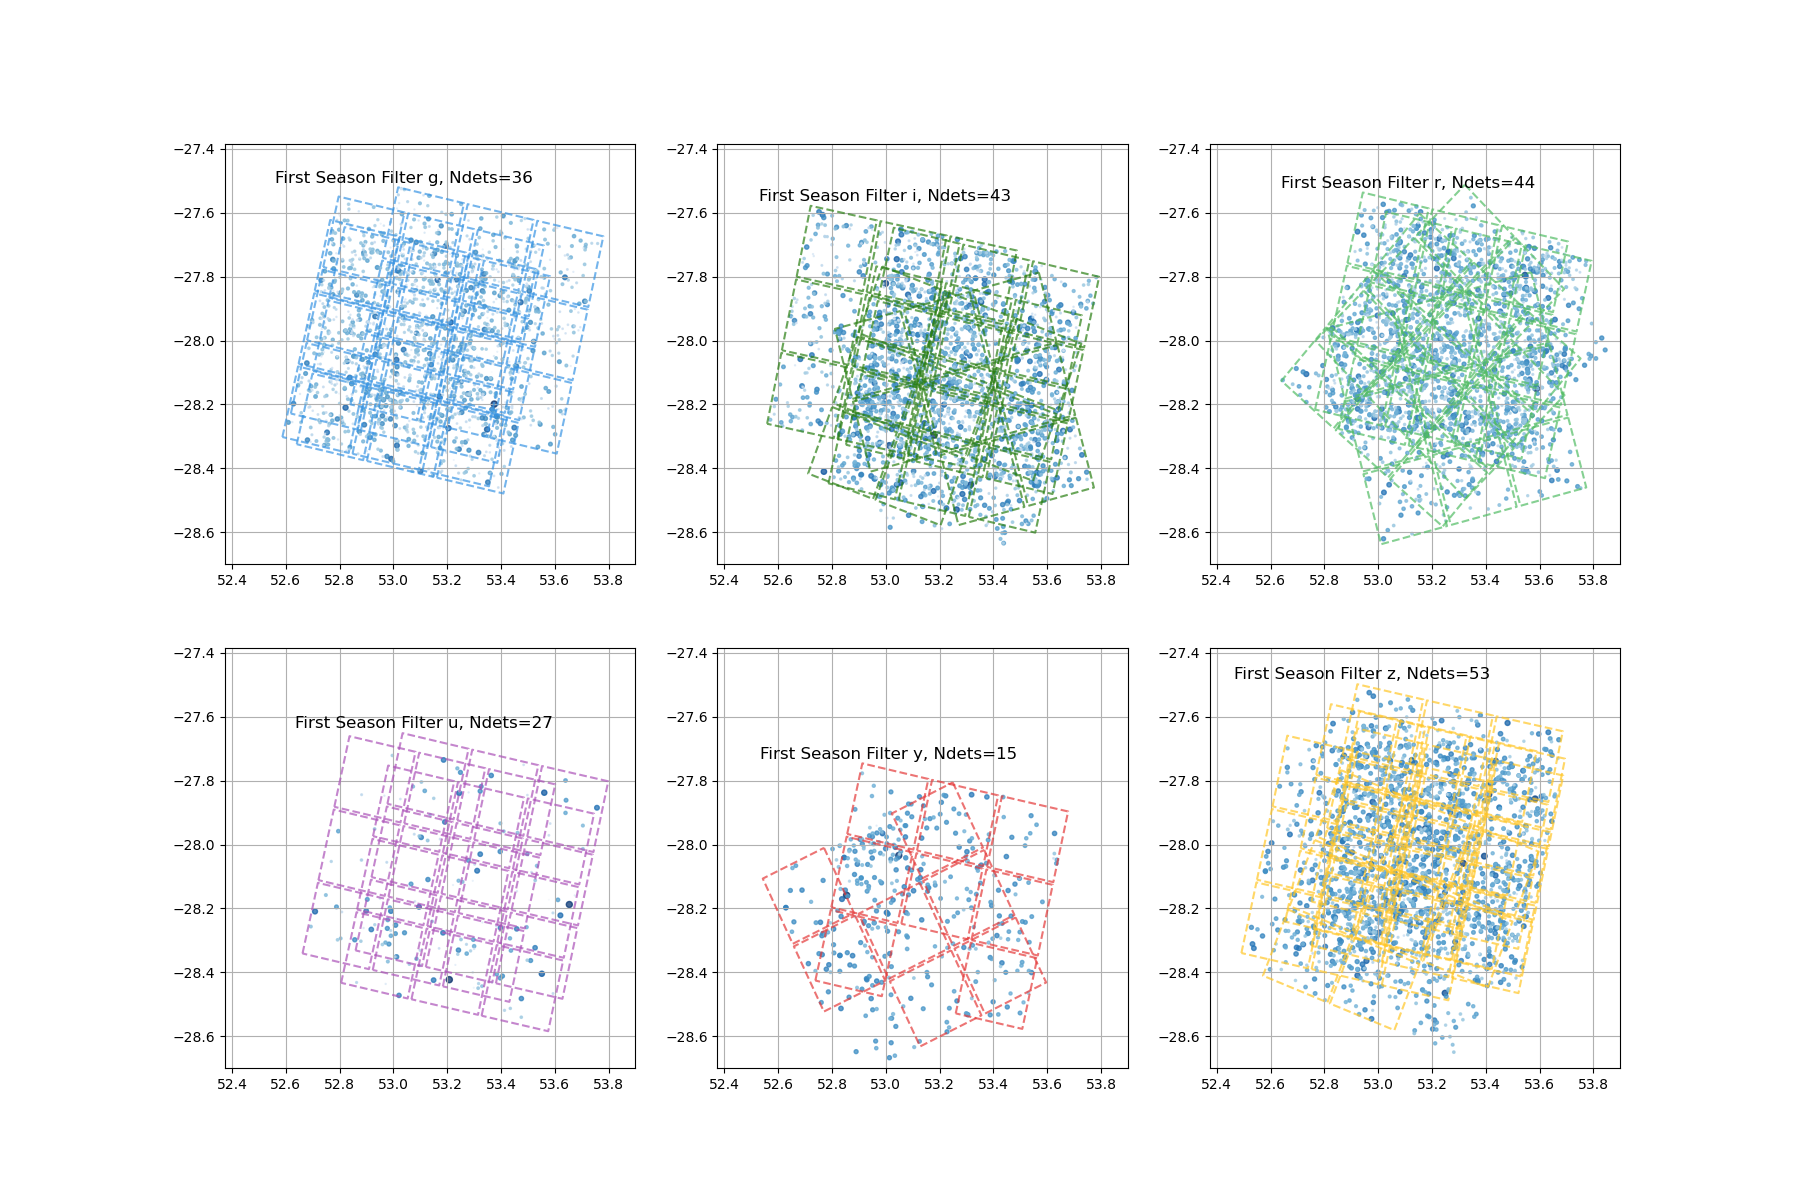
\includegraphics[width=0.95\linewidth]{dia/figures/sampled_df_chip_observations_plusfakes.png}
    \caption{The fake position distribution in sky and in the CCDs footprint per bandpass.}
    \label{fig:sampled_df_chip_observations_plusfakes}
\end{figure}

\begin{figure}
    \centering
    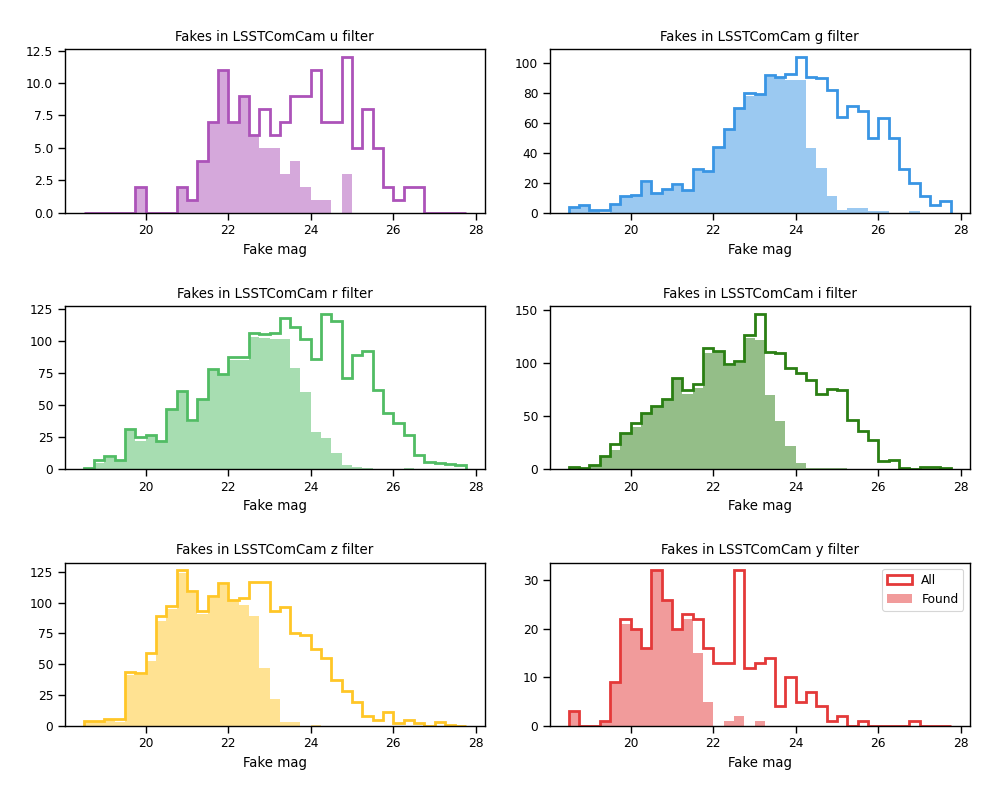
\includegraphics[width=0.95\linewidth]{dia/figures/simple_hist_completeness_mag_per_filter.png}
    \caption{The distribution of magnitudes per bandpass for all the injected fakes (solid lines), and in shaded region the distribution of magnitudes of the fakes detected by the AP pipeline.}
    \label{fig:found_fakes_per_Filter}
\end{figure}


We run Alert Production pipeline with a set of additional tasks that handle fake injection on the \textit{initial\_pvi} images, and then the book-keeping tasks of fake catalog matching to diaSources as well as forced photometry for SNR estimation.

We then, can compile useful statistics about the fake source recovery, that informs us about DIA algorithm performance, as well as detection and measurement algorithm performance. 

For this, we cross-match the position of our candidate detections, or \textit{diaSources} with the positions of the synthetic sources, using a tolerance of $0.5''$ (roughly $2.5$px). 


\begin{figure}
    \centering
    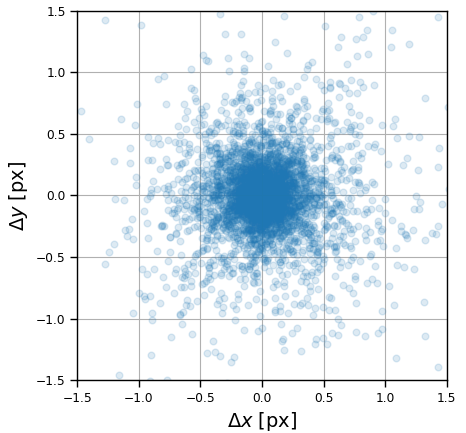
\includegraphics[width=0.49\linewidth]{dia/figures/scatter_xy_diaSrcs_match_px.png}
    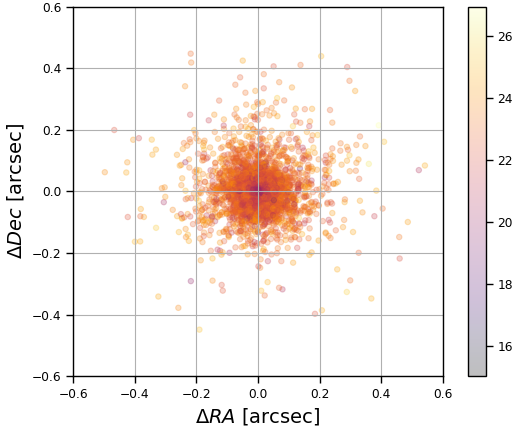
\includegraphics[width=0.49\linewidth]{dia/figures/scatter_radec_diaSrcs_match_arsec_mag.png}
    \caption{The scatter of the coordinate centroid recovery of the fakes. In the left we have the scatter around the true centroid in pixel coordinates, and in the right the scatter around the true center of fakes in sky coordinates (and in units of arc-seconds), wit the grid matching the pixel grid by means of the platescale. Also, we include the brightness in colormap.}
    \label{fig:scatter_radec_diaSrcs_match_arsec_mag}
\end{figure}

Those fakes that found a match are called "found fake" and objects that had no match we refer as "lost" or "missed" fakes. 
The rate of found to existing fakes is our recovery rate, Recall or Efficiency of detection. 

\begin{figure}
    \centering
    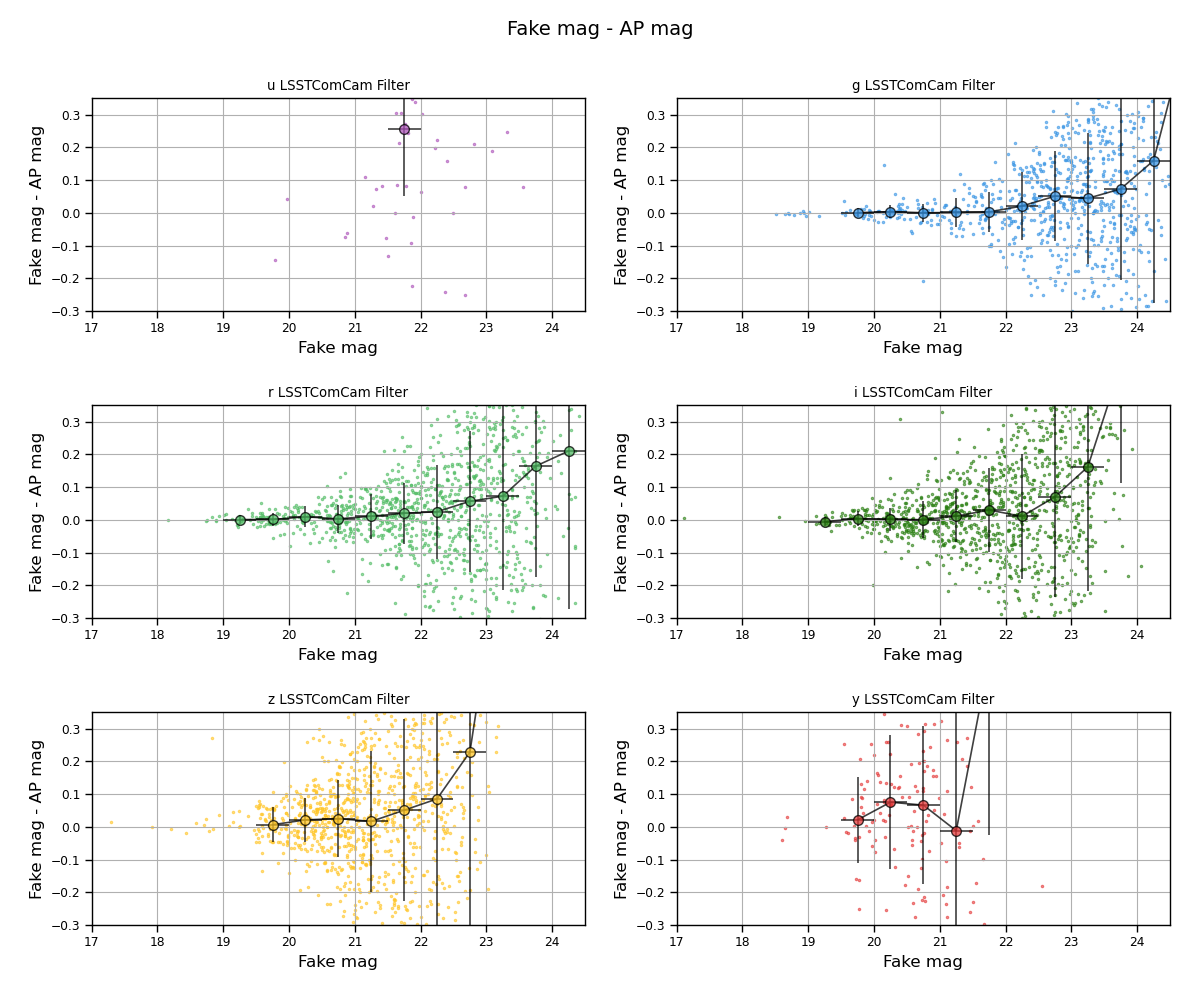
\includegraphics[width=0.95\linewidth]{dia/figures/scatter_mag_ap_mag_perfilter.png}
    \caption{The recovered Aperture magnitude residual per filter for all the found fake sample, as a function of their true magnitude. }
    \label{fig:photometric_recovery_vs_fakemag}
\end{figure}
\begin{figure}
    \centering
    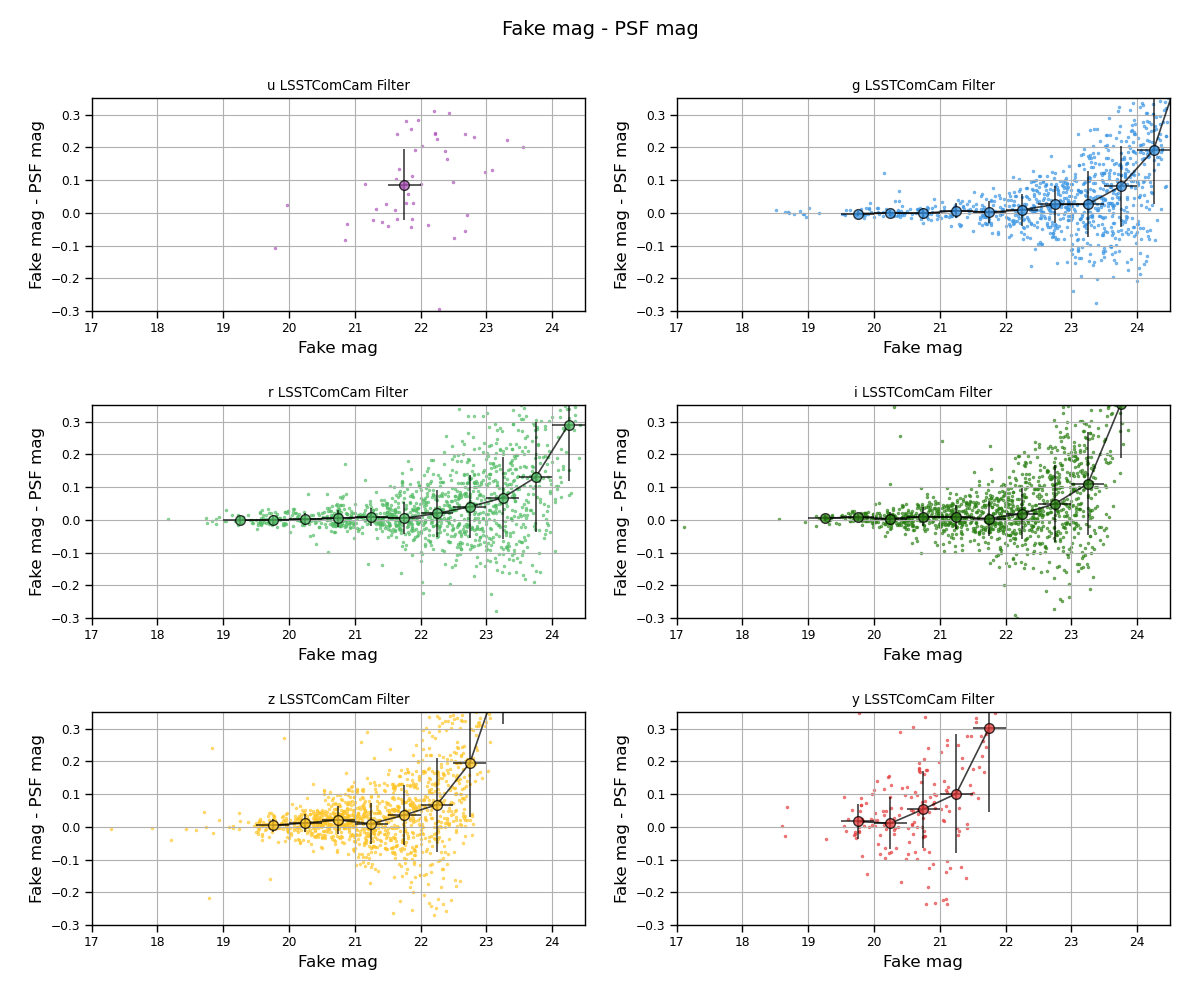
\includegraphics[width=0.95\linewidth]{dia/figures/scatter_mag_psf_mag_perfilter.png}
    \caption{The residual of PSF magnitude measurement for found fakes, as function of their true magnitude.}
    \label{fig:photometric_recovery_psf_vs_fakemag}
\end{figure}
\begin{figure}
    \centering
    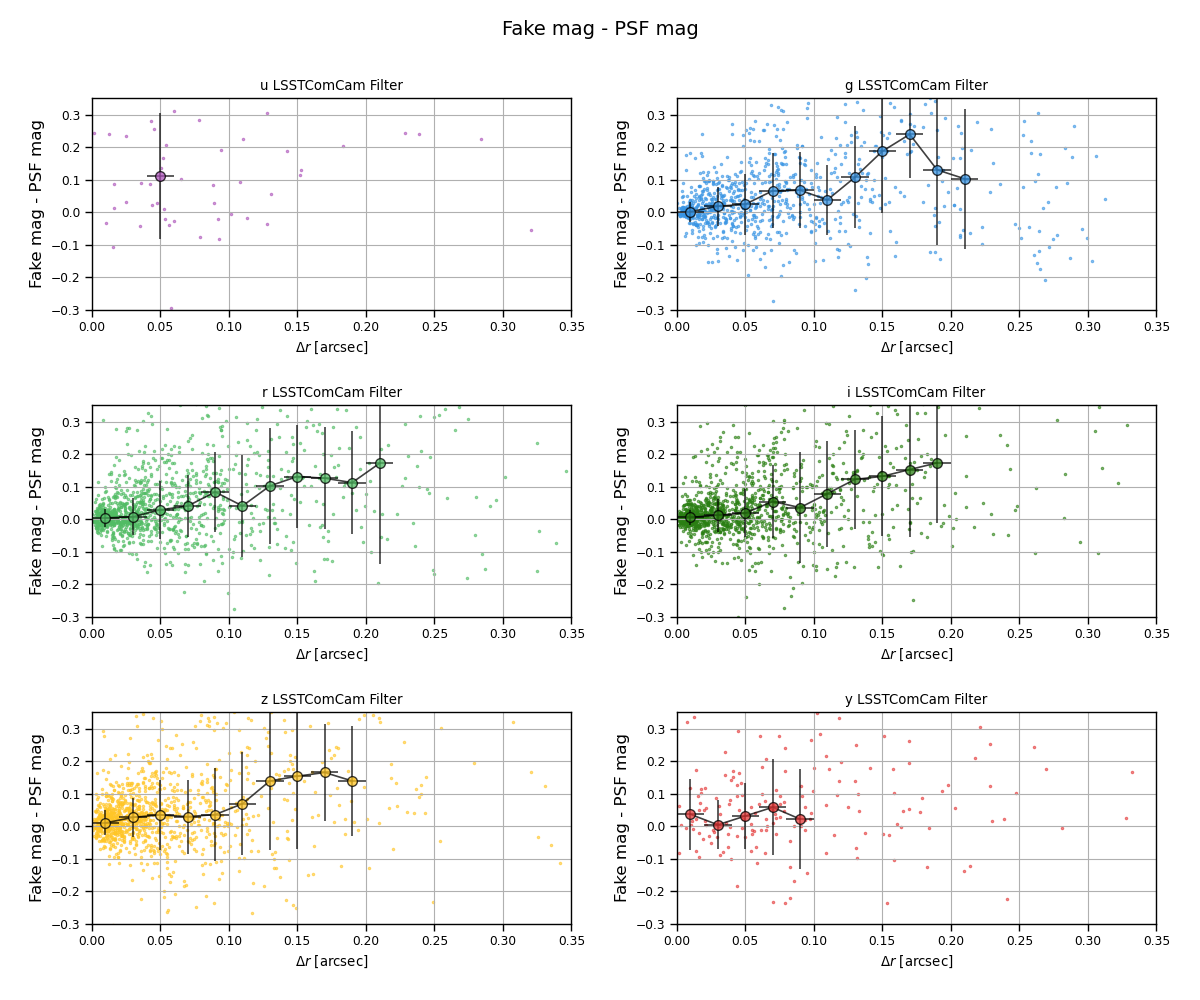
\includegraphics[width=0.95\linewidth]{dia/figures/scatter_dist_psf_mag_perfilter.png}
    \caption{The PSF magnitude residual for the found fakes as function of their matching distance (in [arcsec]).}
    \label{fig:photometric_recovery_vs_astrometric_dist}
\end{figure}

\begin{figure}
    \centering
    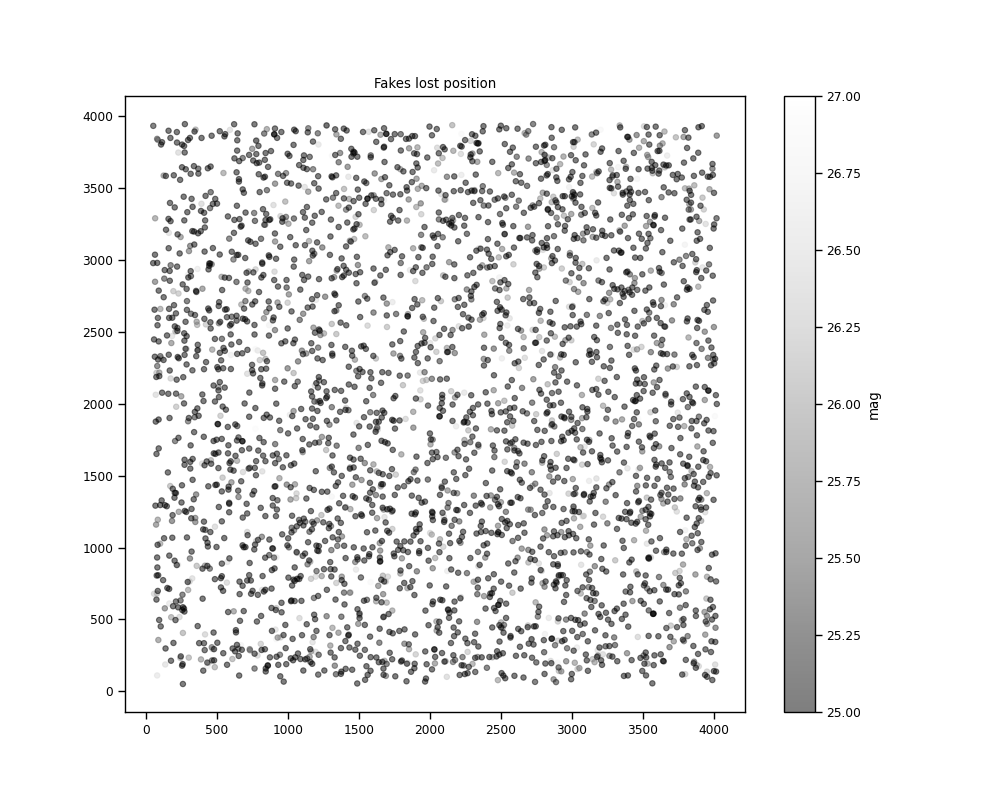
\includegraphics[width=0.95\linewidth]{dia/figures/lost_sources_detector_map.png}
    \caption{The scatter map of the lost sources in the detector coordinates. In gray scale in the colorbar we show the object magnitudes.}
    \label{fig:lost_sources_xy}
\end{figure}


\begin{figure}
    \centering
    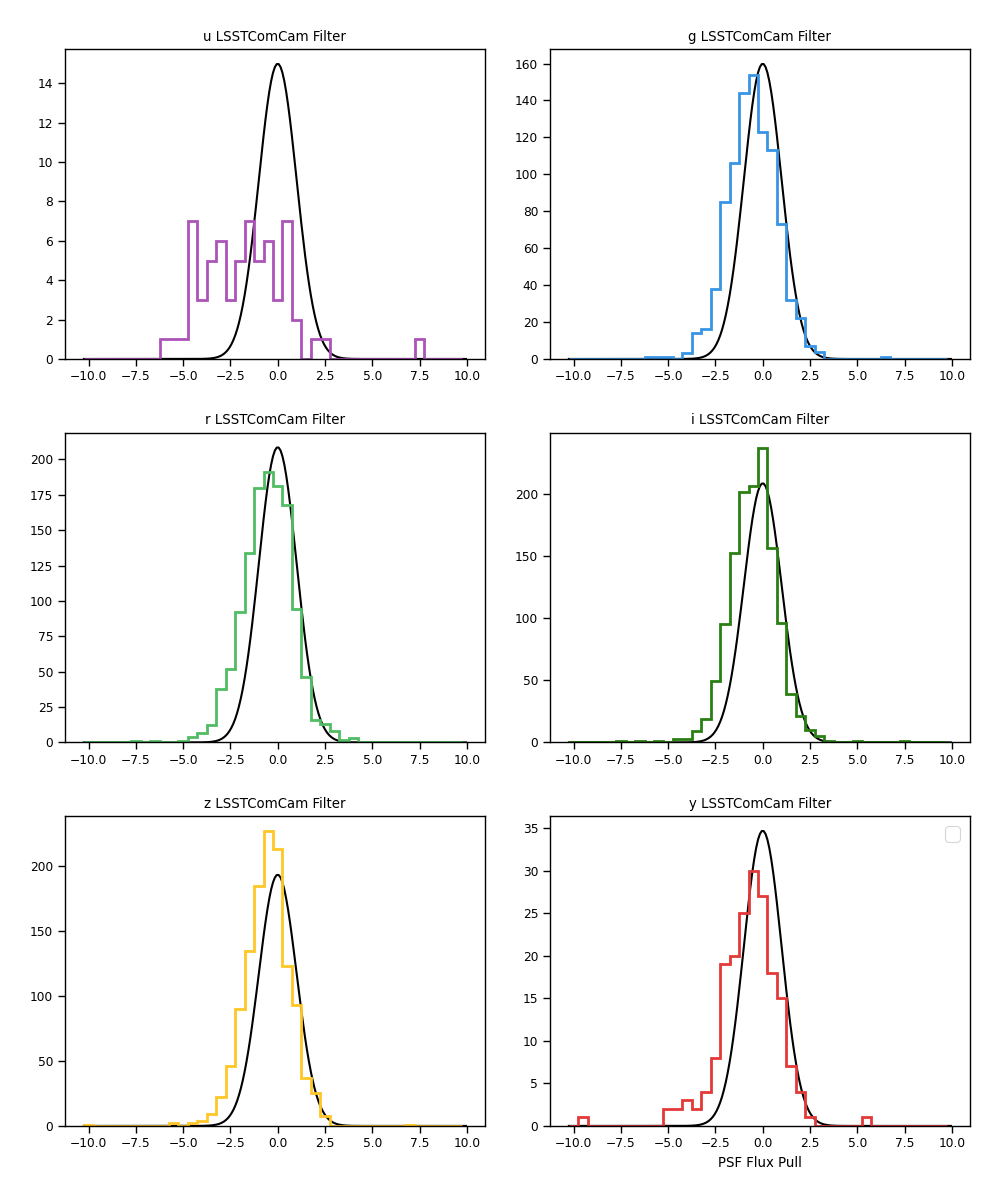
\includegraphics[width=0.95\linewidth]{dia/figures/flux_pulls.png}
    \caption{The flux pull distribution for all the found fakes, in each filter bandpass. A zero mean, unit dispersion Gaussian distribution function is also included for reference.}
    \label{fig:fake_sources_pulls}
\end{figure}


\begin{figure}
    \centering
    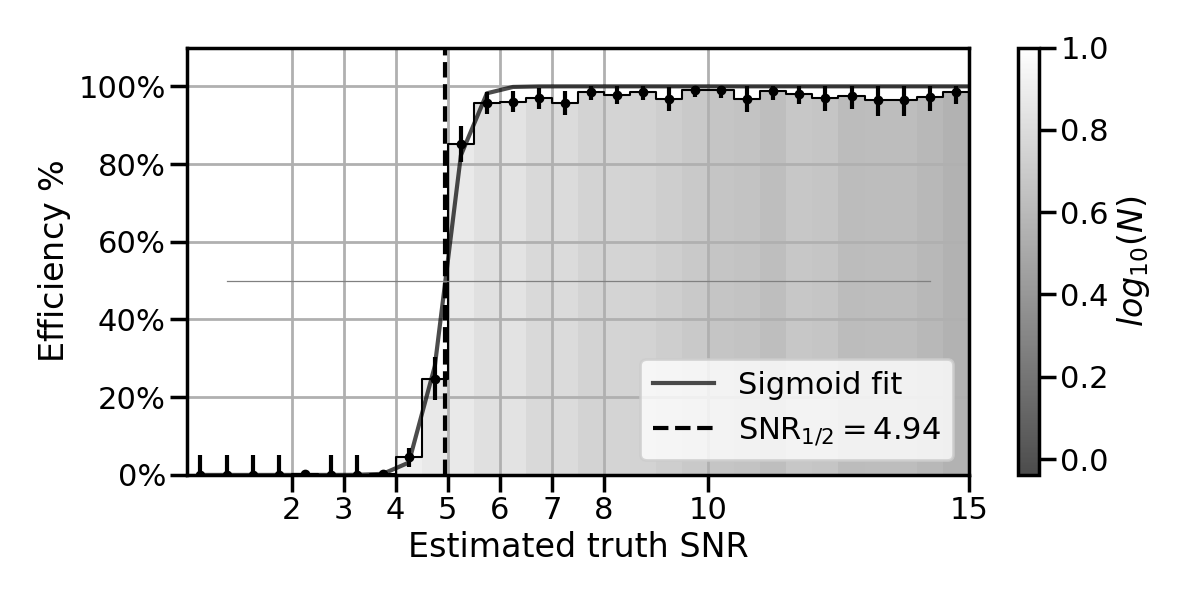
\includegraphics[width=0.95\linewidth]{dia/figures/Efficiency_vs_forced_base_PsfFlux_instFlux_SNR.png}
    \caption{The detection efficiency as function of the PSF estimated S/N ratio of the fake sources. The SNR 1/2 parameter is also included in dashed lines, and represents the 50\% efficiency S/N threshold value (lower is better).}
    \label{fig:eff_vs_snr_fakes}
\end{figure}


